\documentclass[tikz, border=1mm]{standalone}

\usepackage{tikz}
\usetikzlibrary{positioning,shapes,shadows,arrows,fit,decorations.markings,decorations.pathreplacing,calligraphy,calc}

\definecolor{mygreen}{rgb}{0,0.6,0}
\definecolor{mygray}{rgb}{0.5,0.5,0.5}
\definecolor{mymauve}{rgb}{0.58,0,0.82}

\tikzstyle{commonbox}=[rectangle, draw=black, rounded corners, text centered, anchor=north]
\tikzstyle{graybox}=[commonbox, fill=Gray!20]
\tikzstyle{shadowbox}=[commonbox, drop shadow]
\tikzstyle{greenbox}=[shadowbox, fill=YellowGreen!50]
\tikzstyle{apribox}=[shadowbox, fill=Apricot!50]
\tikzstyle{bluebox}=[shadowbox, fill=CornflowerBlue!50]
\tikzstyle{redbox}=[shadowbox, fill=Red!50]
\tikzstyle{blackbox}=[shadowbox, fill=Black!65, text=White]
\tikzstyle{arrow}=[->, -latex, line width=0.8mm, rounded corners=3mm]

\tikzstyle{Data}=[rectangle, draw=blue, text width=35mm, align=center]
\tikzstyle{Tool}=[rectangle, draw=black, fill=white!70!black, text width=35mm, align=center]

\begin{document}
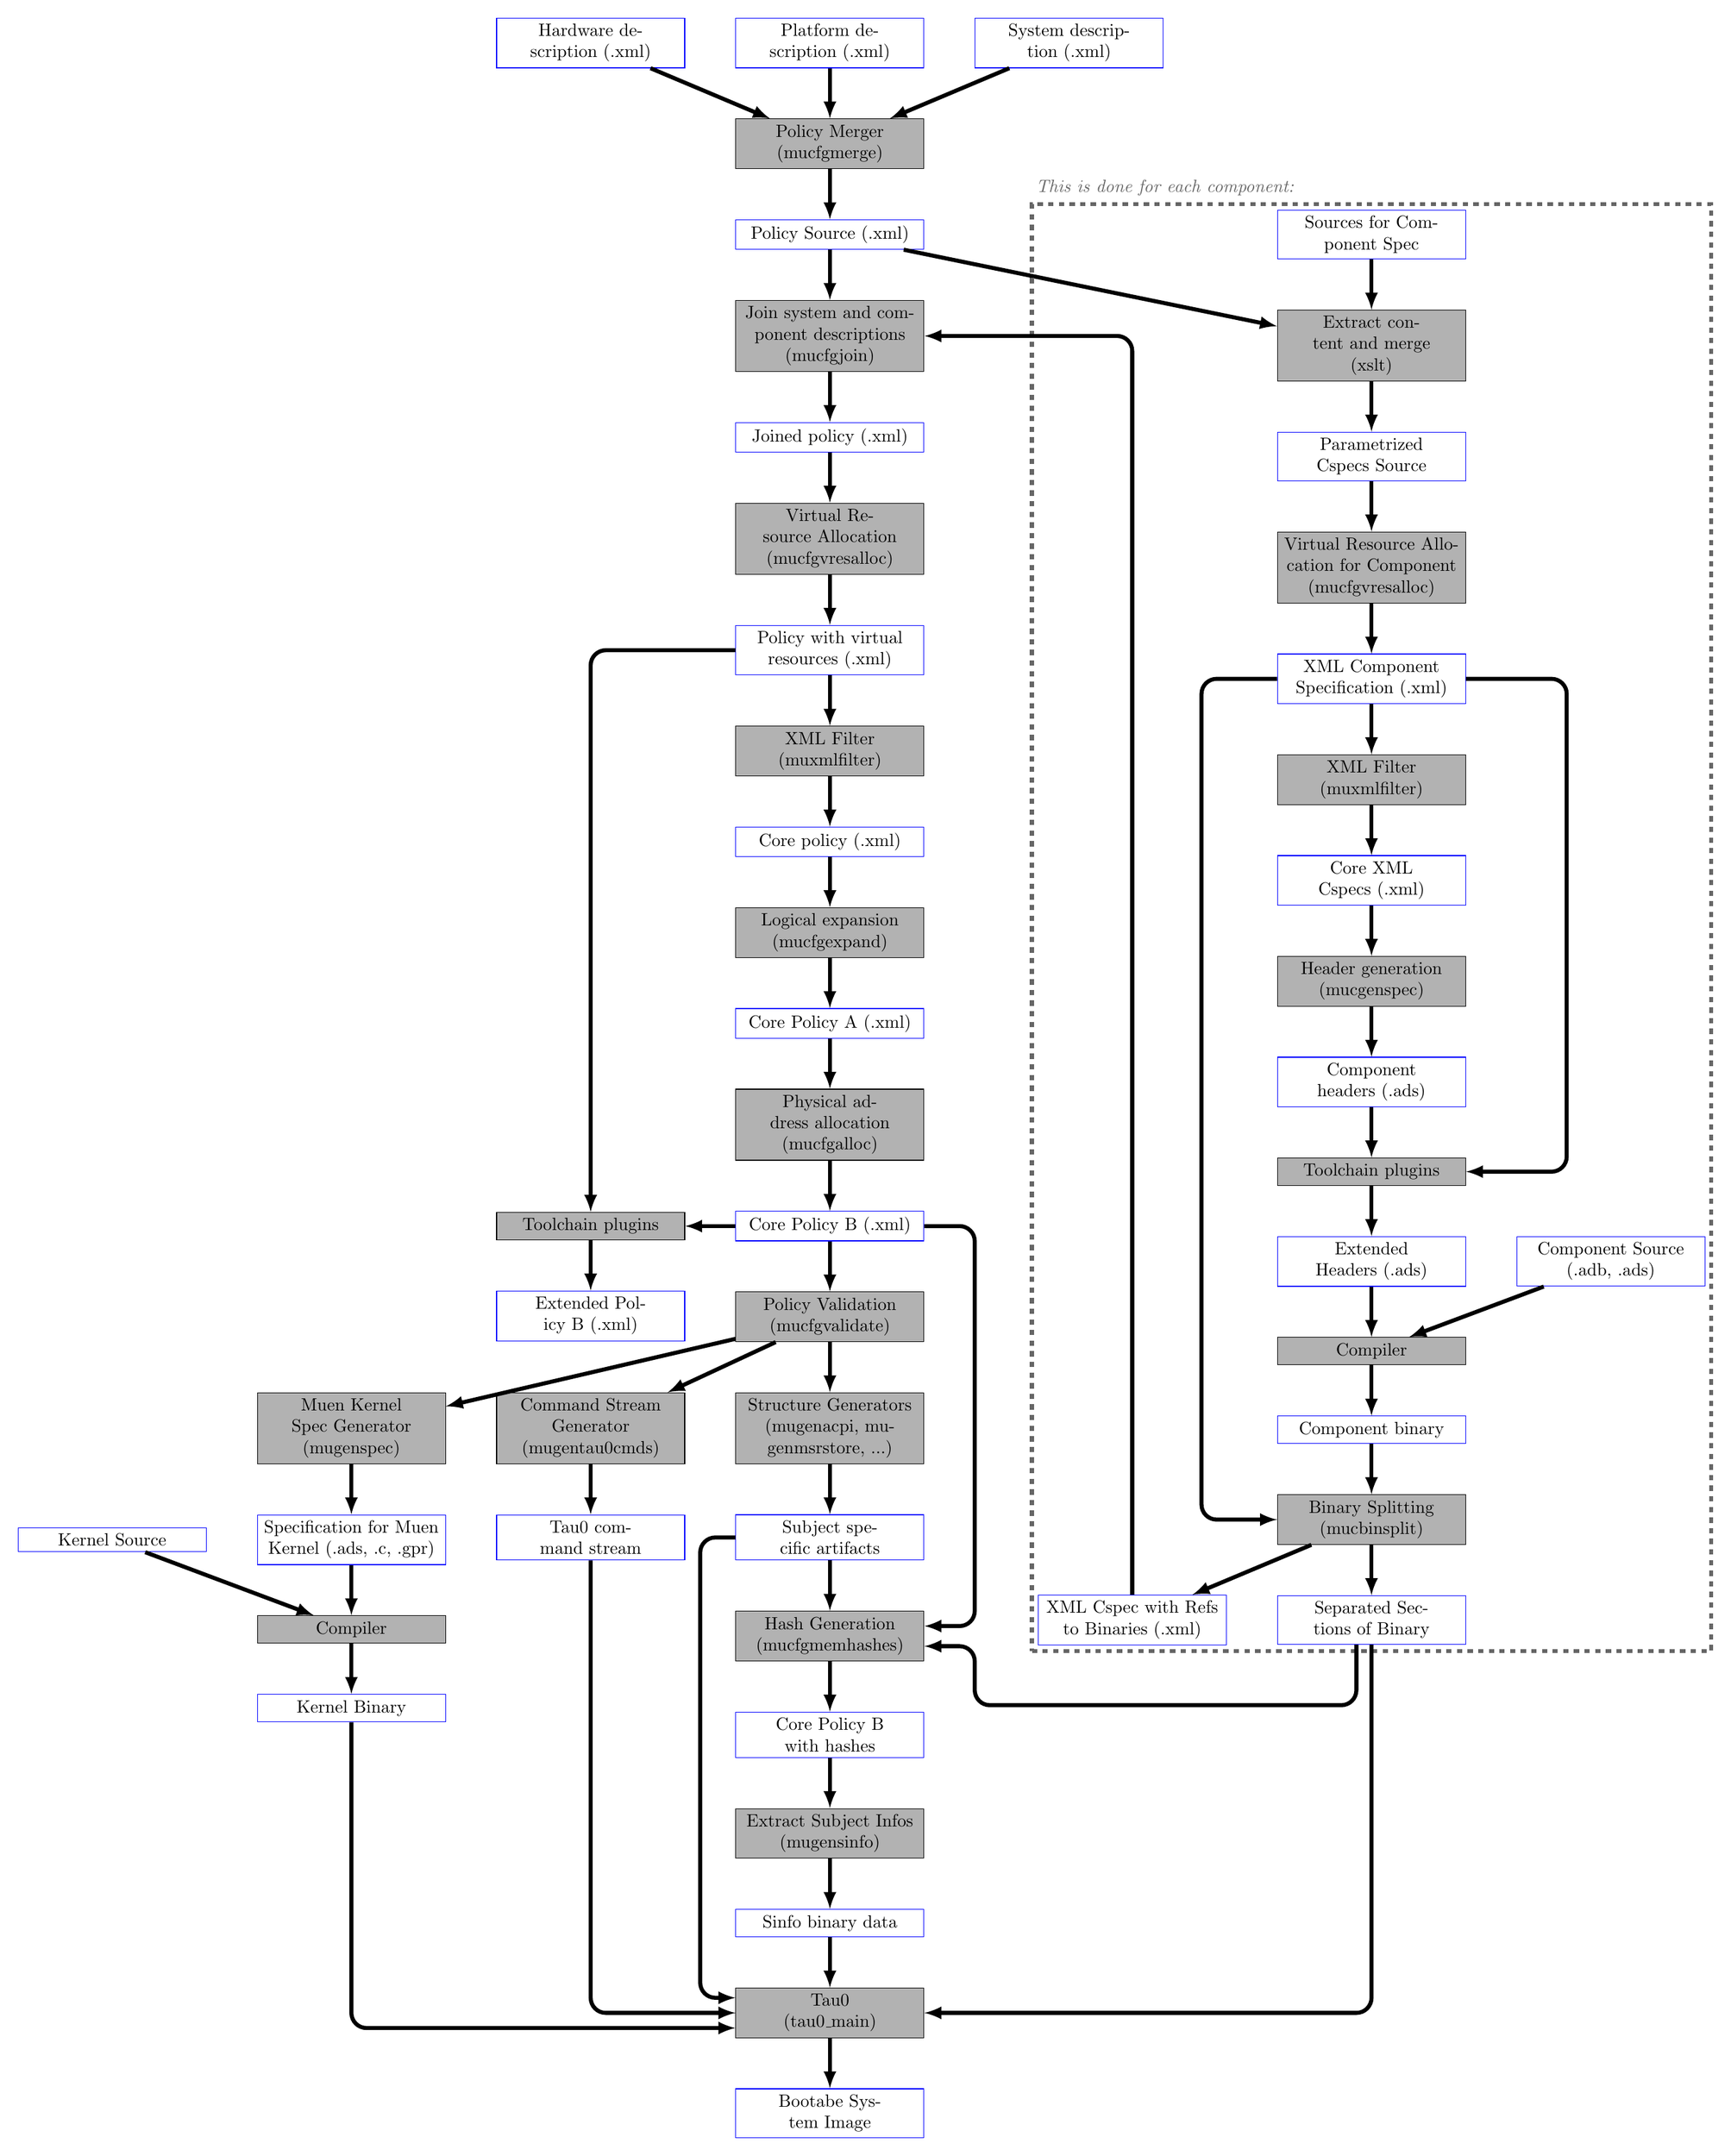
\begin{tikzpicture}
\node [Data] (hardwaresrc) {Hardware description (.xml)};
\node [Data, right= of hardwaresrc] (platformsrc) {Platform description (.xml)};
\node [Data, right= of platformsrc] (systemsrc) {System description (.xml)};

\node [Tool, below= of platformsrc] (mucfgmerge) {Policy Merger\\(mucfgmerge)};
\node [Data, below= of mucfgmerge] (policysrc) {Policy Source (.xml)};
\draw [arrow] (hardwaresrc) to (mucfgmerge);
\draw [arrow] (platformsrc) to (mucfgmerge);
\draw [arrow] (systemsrc) to (mucfgmerge);
\draw [arrow] (mucfgmerge) to (policysrc);

\node [Data, right=70mm of policysrc] (cspecsrc) {Sources for Component Spec};
\node [Tool, below= of cspecsrc] (xsltcspecs) {Extract content and merge\\(xslt)};
\draw [arrow] (cspecsrc) to (xsltcspecs);
\draw [arrow] (policysrc) to (xsltcspecs);

\node [Data, below= of xsltcspecs] (cspecspar) {Parametrized Cspecs Source};
\node [Tool, below= of cspecspar] (mucfgcvresalloc) {Virtual Resource Allocation for Component\\(mucfgvresalloc)};
\node [Data, below= of mucfgcvresalloc] (cspecs) {XML Component Specification (.xml)};
\draw [arrow] (xsltcspecs) to (cspecspar);
\draw [arrow] (cspecspar) to (mucfgcvresalloc);
\draw [arrow] (mucfgcvresalloc) to (cspecs);

\node [Tool, below= of cspecs] (muxmlcfilter) {XML Filter\\(muxmlfilter)};
\node [Data, below= of muxmlcfilter] (cspecvr) {Core XML Cspecs (.xml)};
\draw [arrow] (cspecs) to (muxmlcfilter);
\draw [arrow] (muxmlcfilter) to (cspecvr);

\node [Tool, below= of cspecvr] (mucgenspec) {Header generation\\(mucgenspec)};
\node [Data, below= of mucgenspec] (cspecads) {Component headers (.ads)};
\draw [arrow] (cspecvr) to (mucgenspec);
\draw [arrow] (mucgenspec) to (cspecads);

\node [Tool, below= of cspecads] (cspecplugin) {Toolchain plugins};
\node [Data, below= of cspecplugin] (cspecext) {Extended Headers (.ads)};
\draw [arrow] (cspecads) to (cspecplugin);
\draw [arrow] (cspecplugin) to (cspecext);
\draw [arrow] (cspecs.east) -| ([xshift=20mm]cspecvr.east) |-  (cspecplugin.east);

\node [Data, right= of cspecext] (compsrc) {Component Source (.adb, .ads)};
\node [Tool, below= of cspecext] (compilercspecs) {Compiler};
\node [Data, below= of compilercspecs] (compbinary) {Component binary};
\draw [arrow] (cspecext) to (compilercspecs);
\draw [arrow] (compsrc) to (compilercspecs);
\draw [arrow] (compilercspecs) to (compbinary);

\node [Tool, below= of compbinary] (mucbinsplit) {Binary Splitting\\(mucbinsplit)};
\node [Data, below= of mucbinsplit] (cbinparts) {Separated Sections of Binary};
\node [Data, left= of cbinparts] (cspecwithhash) {XML Cspec with Refs to Binaries (.xml)};
\draw [arrow] (compbinary) to (mucbinsplit);
\draw [arrow] (cspecs.west) -| ([xshift=-15mm]cspecvr.west) |- (mucbinsplit.west);
\draw [arrow] (mucbinsplit) to (cbinparts);
\draw [arrow] (mucbinsplit) to (cspecwithhash);

\node [fit={(cspecwithhash)(compsrc)(cspecsrc)}, draw=white!40!black, dashed, line width=0.8mm] (component_border) {};
\node [above=0mm of component_border.north west, anchor=south west, color=white!40!black] (component_border_text) {\textit{This is done for each component:}};

\node [Tool, below= of policysrc] (mucfgjoin) {Join system and component descriptions\\(mucfgjoin)};
\node [Data, below= of mucfgjoin] (policyjoined) {Joined policy (.xml)};
\draw [arrow] (policysrc) to (mucfgjoin);
\draw [arrow] (cspecwithhash.north) |- (mucfgjoin);
\draw [arrow] (mucfgjoin) to (policyjoined);

\node [Tool, below= of policyjoined] (mucfgvresalloc) {Virtual Resource Allocation\\(mucfgvresalloc)};
\node [Data, below= of mucfgvresalloc] (policyjvr) {Policy with virtual resources (.xml)};
\draw [arrow] (policyjoined) to (mucfgvresalloc);
\draw [arrow] (mucfgvresalloc) to (policyjvr);

\node [Tool, below= of policyjvr] (muxmlfilter) {XML Filter\\(muxmlfilter)};
\node [Data, below= of muxmlfilter] (policyjvrf) {Core policy (.xml)};
\draw [arrow] (policyjvr) to (muxmlfilter);
\draw [arrow] (muxmlfilter) to (policyjvrf);

\node [Tool, below= of policyjvrf] (mucfgexpand) {Logical expansion\\(mucfgexpand)};
\node [Data, below= of mucfgexpand] (policya) {Core Policy A (.xml)};
\draw [arrow] (policyjvrf) to (mucfgexpand);
\draw [arrow] (mucfgexpand) to (policya);

\node [Tool, below= of policya] (mucfgalloc) {Physical address allocation\\(mucfgalloc)};
\node [Data, below= of mucfgalloc] (policyb) {Core Policy B (.xml)};
\draw [arrow] (policya) to (mucfgalloc);
\draw [arrow] (mucfgalloc) to (policyb);

\node [Tool, left= of policyb] (policyplugin) {Toolchain plugins};
\node [Data, below= of policyplugin] (policybext) {Extended Policy B (.xml)};
\draw [arrow] (policyb) to (policyplugin);
\draw [arrow] (policyjvr.west) -| (policyplugin.north);
\draw [arrow] (policyplugin) to (policybext);

\node [Tool, below= of policyb] (validator) {Policy Validation\\(mucfgvalidate)};
\draw [arrow] (policyb) to (validator);

\node [Tool, below= of validator] (structgens) {Structure Generators\\(mugenacpi, mugenmsrstore, ...)};
\node [Data, below= of structgens] (subjectarticfacts) {Subject specific artifacts};
\draw [arrow] (validator) to (structgens);
\draw [arrow] (structgens) to (subjectarticfacts);
%mugenacpi: ACPI tables for VMs
%mugenmsrstore: MSR store regions
%mugenzp: Zero-page regions for VMs
%mugensolo5: Solo5 boot info

\node [Tool, left= of structgens] (mugentau0cmds) {Command Stream Generator\\(mugentau0cmds)};
\node [Data, below= of mugentau0cmds] (commandstream) {Tau0 command stream};
\draw [arrow] (validator) to (mugentau0cmds);
\draw [arrow] (mugentau0cmds) to (commandstream);

\node [Tool, left= of mugentau0cmds] (mugenspec) {Muen Kernel Spec Generator\\(mugenspec)};
\node [Data, below= of mugenspec] (kernelheaders) {Specification for Muen Kernel (.ads, .c, .gpr)};
\draw [arrow] (validator) to (mugenspec);
\draw [arrow] (mugenspec) to (kernelheaders);

\node [Data, left= of kernelheaders] (kernelsource) {Kernel Source};
\node [Tool, below= of kernelheaders] (compilekernel) {Compiler};
\node [Data, below= of compilekernel] (kernelbinary) {Kernel Binary};
\draw [arrow] (kernelheaders) to (compilekernel);
\draw [arrow] (kernelsource) to (compilekernel);
\draw [arrow] (compilekernel) to (kernelbinary);

\node [Tool, below= of subjectarticfacts] (mucfgmemhashes) {Hash Generation\\(mucfgmemhashes)};
\node [Data, below= of mucfgmemhashes] (policybhashes) {Core Policy B with hashes};
\draw [arrow] (subjectarticfacts) to (mucfgmemhashes);
\draw [arrow]  (policyb.east) -| ([shift={(10mm,-10mm)}]policyb.east) |- ([yshift=2mm]mucfgmemhashes.east);
\draw [arrow]  ([xshift=-3mm]cbinparts.south) |-  ([yshift=-12mm]cbinparts.south west) -| ([shift={(10mm,-8mm)}]mucfgmemhashes.east) |- ([yshift=-2mm]mucfgmemhashes.east);
\draw [arrow]  (mucfgmemhashes) to (policybhashes);

\node [Tool, below= of policybhashes] (sinfo) {Extract Subject Infos\\(mugensinfo)};
\node [Data, below= of sinfo] (sinfodata) {Sinfo binary data};
\draw [arrow] (policybhashes) to (sinfo);
\draw [arrow] (sinfo) to (sinfodata);

\node [Tool, below= of sinfodata] (tau0) {Tau0\\(tau0\_main)};
\node [Data, below= of tau0] (img) {Bootabe System Image};
\draw [arrow] (commandstream.south) |-  ([yshift=0mm]tau0.west);
\draw [arrow] (kernelbinary.south) |- ([yshift=-3mm]tau0.west);
\draw [arrow] (subjectarticfacts.west) -| ([shift={(-7mm,-10mm)}]subjectarticfacts.west) |- ([yshift=3mm]tau0.west);
\draw [arrow] (sinfodata) to (tau0);
\draw [arrow] (cbinparts.south) |- ([yshift=-0mm]tau0.east);
\draw [arrow] (tau0) to (img);
\end{tikzpicture}
\end{document}
